\documentclass[UTF8,a4paper,12pt]{ctexart}
\usepackage{caption}
\captionsetup[figure]{name={Fig.}}
\captionsetup[table]{name={Tab.}}
\usepackage{ctex}
\usepackage{amsmath}
\numberwithin{equation}{section}
\allowdisplaybreaks[4]       %多行公式中换页
\usepackage{array}
\usepackage[font=small,font=bf,labelsep=none]{caption}
\usepackage{amssymb}
\usepackage{graphicx} 
\usepackage{tikz}
\usepackage{amsthm}
\usepackage{mathrsfs}
\usepackage{dutchcal}
\usepackage{color}
\usepackage{graphicx}    %插入图片 
\usepackage{times}
\usepackage{mathptmx}
\usepackage{fancyhdr} %页眉页脚
\usepackage{booktabs}  %三线表
\usepackage{mfirstuc}
\usepackage[normalem]{ulem}
\useunder{\uline}{\ul}{}
\pagestyle{fancy}
\fancyhf{}
\fancyfoot[C]{\thepage}
\usepackage{setspace}
\setlength{\baselineskip}{20pt}
\newcommand*{\circled}[1]{\lower.7ex\hbox{\tikz\draw (0pt, 0pt)%
    circle (.5em) node {\makebox[1em][c]{\small #1}};}}
\newcommand\boxcheck{\mbox{\ooalign{$\checkmark$\cr\hidewidth$\square$\hidewidth\cr}}}
\usepackage{hyperref}  %目录
\hypersetup{colorlinks=true,linkcolor=black}
\renewcommand {\thefigure} {\thesection{}-\arabic{figure}}%设定图片的编号。这样设置的实现效果为图1-1
\renewcommand {\thetable} {\thesection{}-\arabic{figure}}
\usepackage{caption}
\captionsetup{font={small},labelsep=quad}%文字5号,之间空一个汉字符位。
\captionsetup[table]{font={bf}} %表格表号与表题加粗
\usepackage{appendix}
\usepackage{tocloft} 
\renewcommand{\cftsecleader}{\cftdotfill{\cftdotsep}} %为目录中section补上引导点
\usepackage{titletoc}
\titlecontents{section}[0pt]{\addvspace{6pt}\filright\bf}%
               {\contentspush{\thecontentslabel \quad}}%
               {}{\titlerule*[8pt]{.}\contentspage}
\makeatletter %双线页眉
\def\headrule{{\if@fancyplain\let\headrulewidth\plainheadrulewidth\fi%
\hrule\@height 1.5pt \@width\headwidth\vskip1.5pt%上面线为1pt粗
\hrule\@height 0.5pt\@width\headwidth  %下面0.5pt粗
\vskip-2\headrulewidth\vskip-1pt}      %两条线的距离1pt
  \vspace{6mm}}     %双线与下面正文之间的垂直间距
\makeatother


\usepackage{titletoc,fmtcount} 
\CTEXsetup[format={\heiti \zihao{3}   \bfseries \center}]{section}
\CTEXsetup[number=Chapter \Numberstring{section}]{section} 

\setmainfont{Times New Roman}



\usepackage[explicit]{titlesec}
\titlespacing*{\section}{0pt}{24pt plus .24pt minus .24pt}{18pt plus .0ex}

\setlength{\headheight}{14.48167pt} 
\setlength{\voffset}{-1.14cm}
\setlength{\topmargin}{0cm}
\setlength{\headsep}{2.9cm}

\begin{document}

\thispagestyle{empty}

\renewcommand{\headrulewidth}{0pt}
\begin{figure}[htb] 
 \center{
\includegraphics[width=5cm]  {fig1.png}} 
 \end{figure}

\begin{center}
\songti \zihao{-2} 上海交通大学学位论文
\end{center}
%该页为中文扉页。无需页眉页脚,纸质论文应装订在右侧
~\\
\begin{center}
\songti \zihao{1} \textbf{基于手势识别与语音识别的安卓网络游戏的设计与开发}
\end{center}
%中文论文标题,1行或2行,宋体,加粗,二号,居中。论文题目不得超过36个汉字
~\\
\begin{center}
\heiti \zihao{4}
\begin{tabular}{l}
\textbf{姓\hspace{1em}名:陈一凡, 陈叙仲, 赖睿奇, 黎泽楷, 易尚霖, 张乐宸}\\
\textbf{学\hspace{1em}号:519370910047, 519021910178, 519021911104}\\
\textbf{\hspace{1em} \hspace{1em} \hspace{1em} 519021910313, 519021910865, 519370910009}\\
\textbf{导\hspace{1em}师:皮宜博}\\
\textbf{学\hspace{1em}院: 密西根学院}\\
\textbf{学科/专业名称:电子与计算机工程}\\
\textbf{申请学位层次:学士学位}\\
\end{tabular}
\end{center}
~\\
\begin{center}
\songti \zihao{4} \textbf{2023年07月}
\end{center}

\newpage
\thispagestyle{empty}
~\\
\begin{center}
\zihao{4}
\textbf{
A Dissertation Submitted to \\
Shanghai Jiao Tong University for Bachelor Degree}
\end{center}
~\\
\begin{center}
\zihao{-2}\textbf{
DESIGN AND DEVELOPMENT OF AN ANDROID ONLINE GAME BASED ON GESTURE RECOGNITION AND SPEECH RECOGNITION}
\end{center}
%英文论文标题:大写,Times New Roman,加粗,14 points,居中
~\\
\begin{center}
\zihao{3} 
Author:  Yifan Chen, Xuzhong Chen, Ruiqi Lai, Zekai Li, Shanglin Yi, Lechen Zhang \\
~\\
Supervisor:  
Yibo Pi
\end{center}
~\\
\begin{center}
\zihao{3} 
University of Michigan –
Shanghai Jiao Tong University
Joint Institute \\
Shanghai Jiao Tong University \\
Shanghai, P.R.China \\
July 31th, 2023  
\end{center}

\newpage
\thispagestyle{empty}
\begin{center}
\heiti \zihao{3}\textbf{
上海交通大学\\
学位论文原创性声明}
\end{center}

\zihao{-4}
本人郑重声明:所呈交的学位论文,是本人在导师的指导下,独立进行研究工作所取得的成果。除文中已经注明引用的内容外,本论文不包含任何其他个人或集体已经发表或撰写过的作品成果。对本文的研究做出重要贡献的个人和集体,均已在文中以明确方式标明。本人完全知晓本声明的法律后果由本人承担。

\begin{flushright}
\begin{tabular}{l}
\zihao{4}
学位论文作者签名:\hspace{20mm}\\
\zihao{4}
日期:\hspace{2em}年\hspace{2em}月\hspace{2em}日
\end{tabular}
\end{flushright}

~\\
\begin{center}
\heiti \zihao{3}\textbf{
上海交通大学\\
学位论文使用授权书}
\end{center}

本人同意学校保留并向国家有关部门或机构送交论文的复印件和电子版,允许论文被查阅和借阅。\\
本学位论文属于 :\par
% use $\boxcheck$ to select the checkbox
$\square$公开论文\par
$\square$内部论文,保密$\square$1年/$\square$2年/$\square$3年,过保密期后适用本授权书。\par
$\square$秘密论文,保密\_\_年(不超过10年),过保密期后适用本授权书。\par
$\square$机密论文,保密\_\_年(不超过20年),过保密期后适用本授权书。\par
(请在以上方框内选择打“√”)\\

\begin{flushright}
\zihao{4}
\begin{tabular}{l l}
学位论文作者签名:\hspace{10mm}\qquad \hspace{100mm}&指导教师签名:\\
日期:\hspace{2em}年\hspace{2em}月\hspace{2em}日 &日期:\hspace{2em}年\hspace{2em}月\hspace{2em}日\\
\end{tabular}
\end{flushright}

\newpage
\pagenumbering{Roman}
\fancyhead[LH]{上海交通大学学位论文}


\addcontentsline{toc}{section}{摘\hspace{1em}要}
\section*{摘\hspace{1em}要}
%摘要:二字间空一格,黑体16磅加粗居中,单倍行距,段前24磅,段后18磅。

本文介绍了一款基于语音识别和手势识别技术的忍者类实时对战游戏Ninja的开发过程和设计思路。该游戏在安卓平台上运行,玩家通过使用手势来放出技能,与对手进行战斗并争夺胜利。我们采用了先进的语音识别和手势识别算法,实现了准确的技能触发和反应速度。此外,游戏还提供了丰富多样的战斗技能,使玩家能够选择适合自己的战斗策略来取得游戏的胜利。值得一提的是,我们利用Unity来打造引人入胜的战斗场景,使玩家在享受游戏胜利的喜悦时,也能够获得出色的视觉体验。通过大量的测试和优化,我们确保了游戏的稳定性和流畅性。实验结果表明,该游戏具有出色的用户体验和娱乐性。本研究在游戏领域中探索语音识别和手势识别应用具有一定的实际意义。

~\\
\textbf{关键词}:语音识别,手势识别,Unity,安卓端APP开发,忍者类对战游戏,实时互动,技能触发,多人对战\\
%关键字:宋体12磅,行距20磅,段前段后0磅,关键字之间用逗号隔开,关键词三个字加粗。

\newpage
\addcontentsline{toc}{section}{ABSTRACT}
\section*{ABSTRACT}
%ABSTRCT:Arial 16磅加粗居中,单倍行距,段前24磅,段后18磅
%\setsansfont{Arial}

This thesis presents the development process and design concept of a real-time ninja battle game, Ninja, based on voice recognition and gesture recognition technologies. The game operates on the Android platform, where players utilize gestures to unleash skills and engage in battles to secure victory. We have implemented advanced voice recognition and gesture recognition algorithms to achieve precise skill triggering and response speed. Additionally, the game offers a diverse range of combat abilities, allowing players to select strategies that suit their fighting style and lead them to triumph. It is worth mentioning that we have utilized Unity to create captivating combat scenes, providing players with a delightful visual experience while enjoying the thrill of game victory. Extensive testing and optimization have been conducted to ensure game stability and smoothness. Experimental results demonstrate that the game offers an exceptional user experience and entertainment value. This research holds practical significance in exploring the application of voice recognition and gesture recognition in the gaming domain.\\
%英文摘要内容:Times New Roman 12磅,行距20磅段前段后0磅
~\\ 
\textbf{Key words}: Voice recognition, gesture recognition, Unity, Android app development, ninja-themed battle game, real-time interaction, skill triggering, multiplayer battles.
%Keywords:Times New Roman 12磅,行距20磅, “key words” 两词加粗



\newpage
\renewcommand\contentsname{\textbf{Content}}

\begin{center}
{\tableofcontents
\thispagestyle{fancy}
\fancyhead [RO, LE] {\normalsize{\songti 第一章\quad绪论}}
\fancyhead [LO, RE] {\normalsize{\songti 上海交通大学学位论文}}
}
\end{center}



\newpage
\fancyhead[LH]{上海交通大学学位论文}
\fancyhead[RH]{Chapter One Introduction}
\pagenumbering{arabic}
\section{Introduction}
\subsection{Background}
With the continuous development of mobile devices and intelligent technologies, mobile gaming has become an integral part of people's everyday entertainment. Among them, real-time battle games have gained popularity among players due to their interactivity and competitiveness. However, traditional real-time battle games often rely on screen touch or button controls, limiting the players' means of control and their overall gaming experience. In order to enhance immersion and entertainment, we aim to develop a ninja-themed real-time battle game based on Android platform, by integrating voice recognition and gesture recognition technologies, allowing players to unleash skills through natural and intuitive movements and sounds, thus achieving a more immersive gaming experience.
\subsection{Problem statement}
In traditional real-time battle games, players control their characters and unleash skills through screen touch or buttons, which may not be intuitive or natural for some players, limiting their control abilities and overall gaming experience. Furthermore, due to the limitations of these control methods, the competitiveness and interactivity of the game are somewhat constrained. Therefore, our challenge is to develop a ninja-themed real-time battle game based on voice recognition and gesture recognition technologies, offering more intuitive and natural control methods, and enhancing the game's competitiveness and interactivity.
\subsection{Existing solutions and their problems}
Currently, there are some experimental games that utilize voice recognition and gesture recognition. However, they may face certain challenges. On one hand, existing solutions may have limitations in terms of accuracy and response speed of skill triggering, leading to delays and imprecise player actions. On the other hand, the variety and personalization of skills and control methods provided in the game may be lacking, failing to meet the diverse needs and combat strategies of players.
\subsection{Proposed solution}
To overcome these challenges, our solution is to develop a ninja-themed real-time battle game based on voice recognition and gesture recognition technologies. By implementing advanced voice recognition and gesture recognition algorithms, we achieve precise skill triggering and response speed, allowing players to control their characters and unleash skills through natural gestures and sounds. Additionally, we provide a diverse range of combat skills, enabling players to choose suitable skill combinations based on their preferences and combat strategies. Through extensive testing and optimization, we ensure the stability and smoothness of the game, delivering an exceptional user experience and entertainment value. We believe that our solution will offer players a fresh gaming experience and explore the potential application value of voice recognition and gesture recognition in the gaming domain.

\newpage
\fancyhead[LH]{上海交通大学学位论文}
\fancyhead[RH]{Chapter Two Design specification}
\section{Design specification}
\subsection{User Interview Questionnaire}
In order to gain a deeper understanding of users' opinions about our game, we have created the following user interview questionnaire.\\

Thank you for participating in our user interview. Please provide your feedback and opinions on our ninja-themed real-time battle game based on voice recognition and gesture recognition technologies. Your answers will be invaluable in further improving and optimizing our game.

\subsubsection{About Ninja(Naruto)'s memory/impression}
\begin{enumerate}
    \item What's impression on Ninja/Naruto?
    \item Talk about your impression about how ninja fight with each other?
    \item What do you feel if you can simulate ninja’s actions in Naruto  in a game?
    \item Have you found any game that can simulate ninja's in your memory/expression?
\end{enumerate}
\subsubsection{About Game Platforms}
\begin{enumerate}
    \item Could you share your gaming habits on mobile phones? For example, what types of mobile games do you prefer, and how often do you play games on mobile phones?
    \item What is your past experience of entertainment (e.g. games, videos) on the theme of Ninjas? What do you most appreciate and expect from them? 
    \item What style do you think would be suitable or do you prefer in such type of game? (e.g. pixel art or anime, font, user interface, etc.)
\end{enumerate}
\subsubsection{About Voice/Gesture Recognition}
\begin{enumerate}
    \item What kinds of limitations in gesture recognition and voice recognition have you experienced?
    \item Our game will be based on the theme of ninja and use gesture and voice recognition. What do you expect from this combination? 
    \item Have you ever used or seen any software with gesture recognition, on mobile phones in particular?
\end{enumerate}

Thank you for taking the time to answer the above questions. Your opinions are highly valuable to us. If you have any additional comments or thoughts you would like to share, please feel free to do so below.

Thank you for your participation!

\subsection{Customer interviews}
To gather comprehensive feedback and understand various users' perspectives on our app, we conducted interviews with 10 users and compiled the following result:

\subsubsection*{Participant1:} 
I have never watched Naruto.

I know little about how ninja fight with each other.

I think it would be a fantastic game and I will have a try. I have never experienced such game before.

I prefer Honor of Kings and PUBG

I think Fighting game is not comfortable on mobile phones

PC game is inconvenient both on time and place, so I prefer mobile game
Don't have any preference on mobile game's art style

Prefer third-person view games rather than platform 2D games.

I have only experienced gesture control in screen, like in ipone, never experienced any games with such feature.

Mac has gesture capture, but only can reconginize fingers.

For voice recognition, I have only used on siri, not for entertainment usage.

Capture recoginition might be not flexible enough, it will definitely influence user experience.

\subsubsection*{Participant2:} 
I still remeber the anime Naruto, it is one of the favorite animes in my life.

My memory about ninja is that they can use a lot of skills shouting out the skill names

I think it would be cool ninja-theme game is an online game.

I prefer the game's art style to be 3D.

I never played any games with gesture capture.

I only experienced voice recoginition in Siri.

I prefer mobile games rather than PC games for they are cheap

I expect the ninjas can move around and play perform their skills with player's voice.

Don't know how to control characters with gesture.

\subsubsection*{Participant3:} 
I of course know Naruto. I like it very much.

My impression about ninjas' fighting is that they use cool and colorful skills in the war.

I would appreciate such game for players to fight as a ninja.

I like to play card games on mobile phones since they don't take a lot of time.

I've heard of there's a mobile phone game directly realted to Naruto, but I've never played it.

I prefer fantasy art style.

Add AR and GPS: like PokemanGo.

I expect the game with AR/VR can have features such as Sociality.

I've experienced two voice recognition software: Xunfei for meeting recording and Sonic for audio to text software.

I've experienced Gesture Recoginition software: Huawei gesture recoginition.

\subsubsection*{Participant4:}
I don't konw much about Naturo, only know that there are many very powerful ninja, able to use powerful ninjutsu

Different ninjas use their own jutsu to defeat the enemy

I think the game with ninja-theme is interesting, never thought it before.

Didn't know whether games with ninja-theme exist

Prefer 王者荣耀or和平精英, play it everyday

No experience on games about Naturo before,  would expect some interesting way of fighting

I would expect like real fight, not just like cards fight

I think the potential disadvantages of the gesture and voice recogintion is that they are not usually as accurate as expected

Would be interested in such game, seems interesting and never played before.

In memory, no, only know some AR games popular like Pokemon go

\subsubsection*{Participant5:}
The most impressive is Sasuke's apparent wheel eyes.

Ninjas use Ninjutsu to defeat the enemy

Would be interested in it! and want to have a try

Never heard of games related to Ninja, only know some card game about Njnja

I only play PC games like CSgo and Pubg, don't play mobile games at all
past experience is like 10 years ago, card games, similar to 梦幻西游, card games, most interseting thing about them is that they have many ninjutsus

Like RPG mode is prefered, I can be a ninjutsu myself and fight

There are hardware limitions, and in many situations they are not practial to use

Would expect different kinds of cool ninjutsus.

No such game seen before

\subsubsection*{Participant6:}
A very classic Japanese anime, several hundred episodes

Ninjas use Ninjutsu to defeat the enemy

Sounds great, and would have a try

Ninja-theme game would be very cool, and interesting

Never heard of such kind of game, and no experience on games based on topic of Ninja

Like casual games, such as subway parkour, play games when boring or on the train and without internet

would prefer Self-playing chess or something like that

not very practical, seems cannot be used in noise situations like when on the subway

Would expect different kinds of cool ninjutsus.

\subsubsection*{Participant7:}
Haven't heard about Naruto ever

My impression on how ninja's fight with each other is that they perform different gestures for different use.

It will be interesting to have a try with a game related to ninja and gesture recongnition.

No such a game with ninja theme

Honor of kings is the favorite one which is PVP and simple

Hope it will be easy to learn and requires less time to finish a round

Of course anmine with good-looking actors

Gesture recognition is often frame-based instead of video streaming based.

I would expect both of gesture and voice recogntion could be utilized well

Have heard of some games on gesture control but don't have a deep impression.

\subsubsection*{Participant8:}
Naruto is an impressive design in Japanese animation

Ninjas use different combination of skills to attack others

A good idea to combine voice and gesture recognition, willing to have a try

No such a game with ninja related topic.

I prefer game that cost a few time to complete a round

I would expect your game to have various mode and enough exploration space

I have no spectial preference for game's art style.

Practical use on mobile app is hardly seen

Will be able to capture gesture accurately is enough

I have never heard of apps with gesture and voice recognition.

\subsubsection*{Participant9:}
Naruto is my favorite Janpanese anime

Various gesture categories and fantastic performances

I would be happy to have a try with game related to ninja.

Haven't heard of such game with ninja theme.

Easy to begin a round like heartstone and interesting to keep playing

Hope it will be able to recognize some interesting gesture and reasonable matching rules

For art style, I think anime will be better

Speech recognition application is widely used in loT but gesture recognition is not used widely

Combination of both modal recognition will be a novelty

No such an app with gesture recognition.
\subsubsection*{Participant10:}
Used to see in a lot of video cut for Naruto.

A very special and impressive competition way.

Worth trying for a game as you described.

No such a game with ninja theme.

PUBG is most usually played, it is easy to begin and worth exploration

Friendly to beginners but have large improvement space for advanced players

Anime art style.

Seems no game app use either techniques(voice and gesture recognition)

The application of either technique on games is attractive enough

No such an app with gesture recognition.
\subsection{Affinity map}
Based on the data that we have collected from the interview, we draw the affinity map that is shown below:
\begin{figure}[htb] 
\center{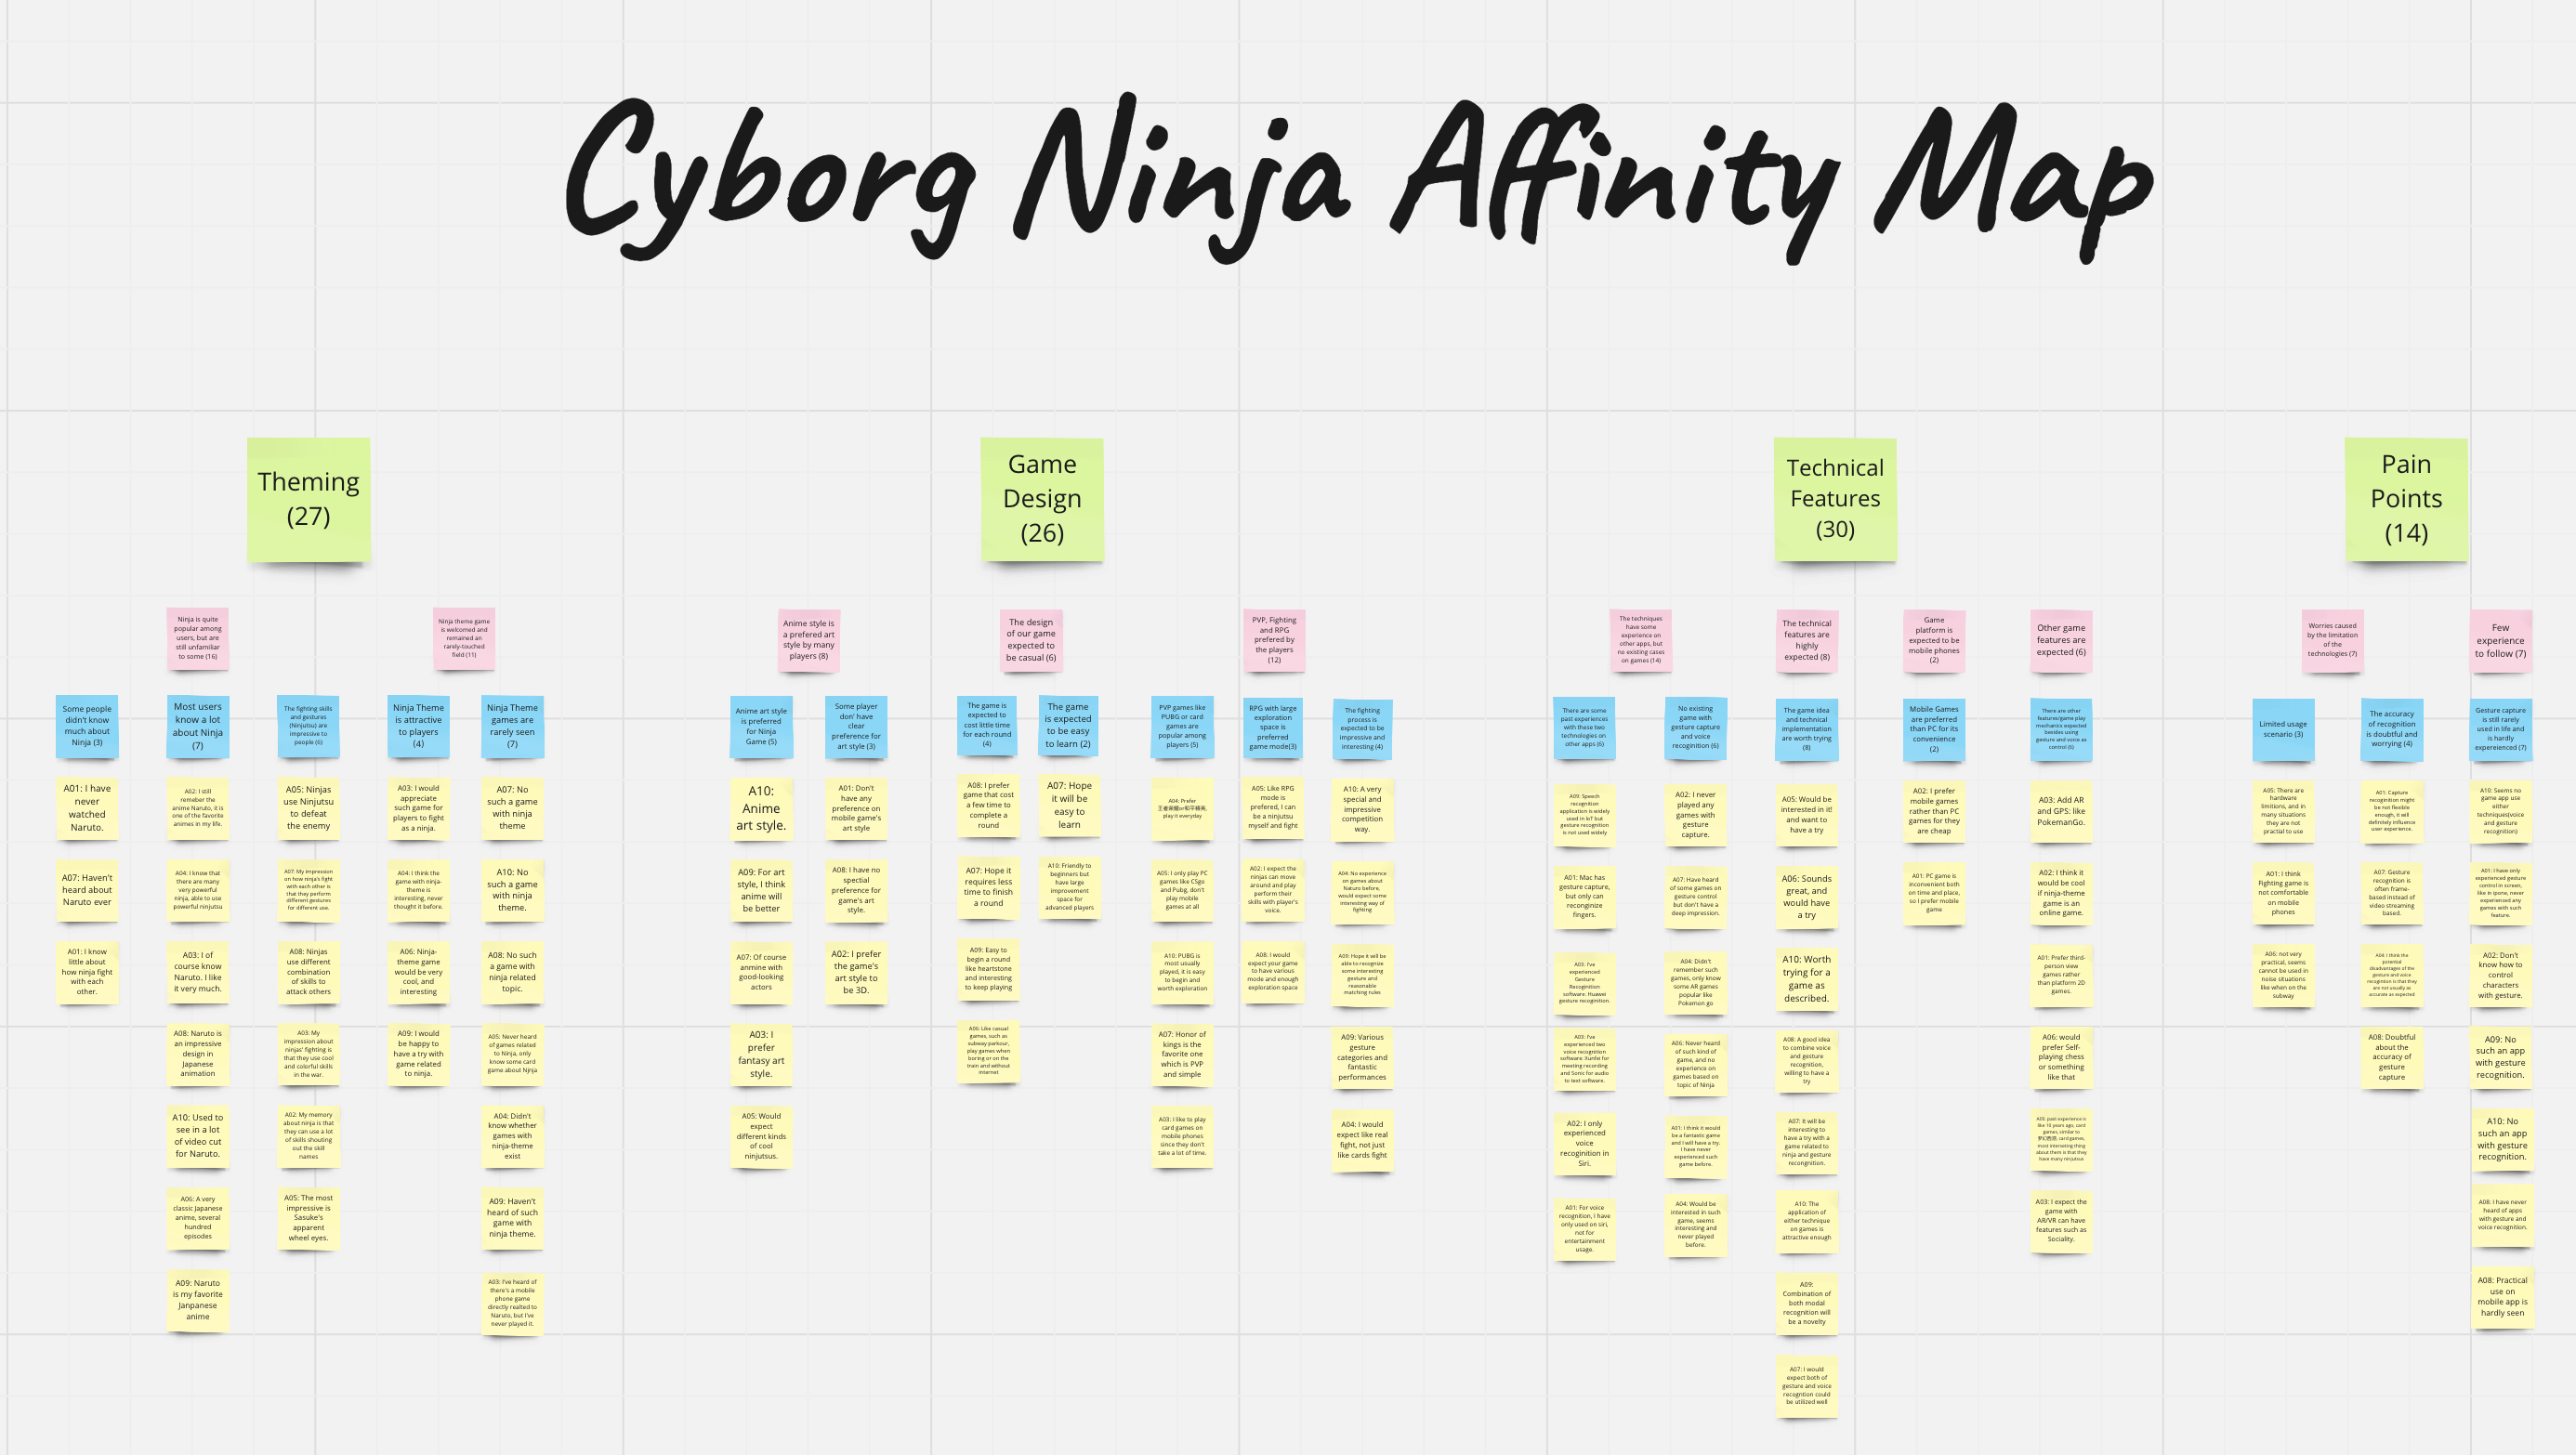
\includegraphics[width=1.0\textwidth]  {Affinity_map.png}} 
\caption{Affinity Map}
\end{figure}
\subsection{Customer profile}
Based on the affinity map, we get the following customer profile:
\subsubsection*{Preference}
\begin{figure}[htb] 
\center{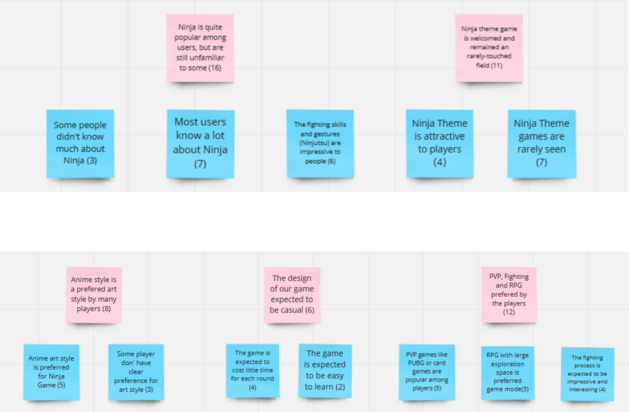
\includegraphics[width=0.7\textwidth]  {preference.png}} 
\caption{Customer's preferences}
\end{figure}
\subsubsection*{Pain Points of customers}
\begin{figure}[htbp] 
\center{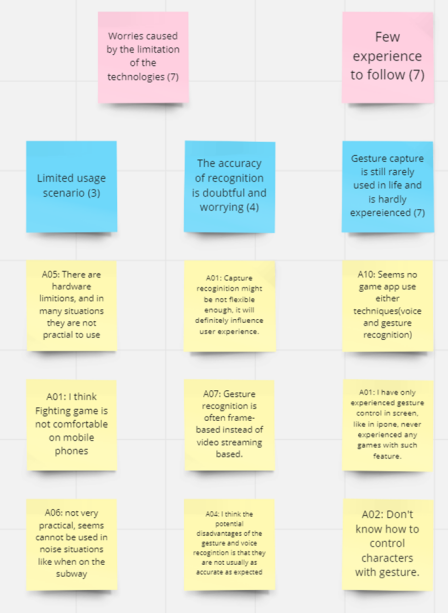
\includegraphics[width=0.35\textwidth]  {pain_points.png}} 
\caption{Pain Points of customers}
\end{figure}

\subsection{Competitor analysis}
After conducting extensive market research, we have identified several similar games and summarized some of their key features.
\subsubsection*{Pokemon Go}
Pokemon Go is an AR mobile app that is based on pokemon collection, and is one vs. one battle. The strength of Pokemon Go is AR, abundant gameplay and artwork, the weakness of it is the ordinary interactive mechanism.

\subsubsection*{Scream Go Hero}
This is a mobile app that use the volume of the player's voice to control the character (a ninja in particular). The strength of it is the interesting mechanism using volume as control, the weakness of it is there are rather too few contents.

\subsubsection*{Words follow the speaker's intent(言出法随)}
This is a pc game, users speak out names of moves to release the characters in the game, the strength of this game is for the interesting mechanism using voice recognition, the weakness of it is the poor gameplay and artwork.

\subsubsection*{Hand Music}
This is an iOS app that can recognize position of hands to play music, the strength of this game is the hand recognition, the weakness of this game is that it is hardly a complete product.

\subsubsection*{Silhouette}
This is a VR app that is able to recognize gesture for all kinds of interaction, the strength of it is for very interesting mechanism using gesture recognition, the weakness of this app is that a VR device is needed.

Based on the competitor analysis, we can get the following table:

\begin{table}[]
\resizebox{\linewidth}{!}{
\begin{tabular}{|c|c|c|c|c|c|}
\hline
               & Gesture Recognition & Voice Recognition & Abundant Gameplay & Extra Feature & Mobile app(no extra device needed) \\ \hline
Pokemon Go     & N                   & N                 & Y                 & Y(AR)         & Y                                  \\ \hline
Scream Go Hero & N                   & Y(only volume)    & N                 & N             & Y                                  \\ \hline
言出法随           & N                   & Y                 & N                 & N             & N                                  \\ \hline
Hand Music     & Y(only hand )       & N                 & N                 & N             & Y                                  \\ \hline
Silhouette     & Y                   & N                 & Y                 & N             & N                                  \\ \hline
Ninja          & Y                   & Y                 & N                 & Y(Unity)      & Y                                  \\ \hline
\end{tabular}
}
\end{table}

\subsubsection*{Conclusion}
 As the table shows, none of the game listed above can satisfy all the needs for customer needs, only our Ninja game has all the features include: Gesture Recognition, Voice Recognition, abundant gameplay content, extra features and also, our game is based on a mobile platform and no need for extra device. Therefore, we have sufficient confidence in our app to perform well in the market.


\newpage
\fancyhead[LH]{上海交通大学学位论文}
\fancyhead[RH]{Chapter Three App Design}
\section{App Design}
\subsection{User Experience Flow and Features}


\subsection{Defining Acceptance criteria for features}

\subsection{Engine Architecture}
......
\subsection{Initial API design}
......
\subsection{UI/UX mockups}
......
\subsection{Usability Testing}
......
\subsection{Final UI/UX design}
......

\newpage
\fancyhead[LH]{上海交通大学学位论文}
\fancyhead[RH]{Chapter Four App development}
\section{App development}

\subsection{Front-end development}
......

\subsection{Back-end development}
......

\subsection{Checking features against acceptance criteria}
......

\newpage
\fancyhead[LH]{上海交通大学学位论文}
\fancyhead[RH]{Chapter Five Discussion and Conclusions}
\section{Discussion and Conclusions}

\subsection{Discussion}
......

\subsection{Conclusion}
......

\subsection{Future Works}
......

\newpage
\fancyhead[LH]{上海交通大学学位论文}
\fancyhead[RH]{Acknowledgements}

\addcontentsline{toc}{section}{Acknowledgements}
\section*{Acknowledgements}

……

\newpage
\fancyhead[LH]{上海交通大学学位论文}
\fancyhead[RH]{References}

\addcontentsline{toc}{section}{References}
\renewcommand\refname{References}
\begin{thebibliography}{1}
\bibitem{1} 杨瑞林, 李力军. 新型低合金高强韧性耐磨钢的研究[J]. 钢铁. 1999(7): 41-45.
\bibitem{2} 于潇, 刘义, 柴跃廷, 等. 互联网药品可信交易环境中主体资质审核备案模式[J]. 清华大学学报(自然科学版), 2012, 52(11): 1518-1523.
\bibitem{3} Schinstock D.E., Cuttino J.F. Real time kinematic solutions of a non-contacting, three dimensional metrology frame[J]. Precision Engineering. 2000, 24(1): 70-76. 
\bibitem{4} 温诗铸. 摩擦学原理[M]. 北京: 清华大学出版社, 1990: 296-300.
\bibitem{5} 蒋有绪, 郭泉水, 马娟, 等. 中国森林群落分类及其群落学特征[M]. 北京: 科学出版社, 1998: 5-17.
\bibitem{6} 贾名字. 工程硕士论文撰写规范[D]. 上海: 上海交通大学, 2000: 177-178.
\bibitem{7} 张凯军. 轨道火车及高速轨道火车紧急安全制动辅助装置: 201220158825.2[P]. 2012-04-05.
\bibitem{8} 全国信息与文献标准化技术委员会. 文献著录: 第4部分 非书资料: GB/T 3792.4-2009[S]. 北京: 中国标准出版社, 2010: 3.
\end{thebibliography}%(参考文献格式请参考GB/T 7714-2015《信息与文献 参考文献著录规则》)

\newpage
\fancyhead[LH]{上海交通大学学位论文}
\fancyhead[RH]{Appendix1}

\addcontentsline{toc}{section}{Appendix}
\section*{Symbols and Marks Appendix 1}

\newpage
\fancyhead[LH]{上海交通大学学位论文}
\fancyhead[RH]{Appendix2}

\addcontentsline{toc}{section}{Appendix2}
\section*{Symbols and Marks Appendix 2}



\newpage
\pagenumbering{arabic}
\fancyhead[LH]{上海交通大学学位论文}
\fancyhead[RH]{}
\section*{NUMERICAL SIMULATION OF HOMOGENEOUS CHARGE COMPRESSION IGNITION COMBUSTION FUELED WITH DIMETHYL ETHER}%英文大摘要标题

HCCI (Homogenous Charge Compression Ignition) combustion has advantages in terms of efficiency and reduced emission. HCCI combustion can not only ensure both the high economic and dynamic quality of the engine, but also efficiently reduce the NOx and smoke emission. Moreover, one of the remarkable characteristics of HCCI combustion is that the ignition and combustion process are controlled by the chemical kinetics, so the HCCI ignition time can vary significantly with the changes of engine configuration parameters and operating conditions. ……%(英文大摘要正文)



\end{document} 